\chapter[Modelação]
{Modela\c{c}\~ao}

Após o levantamento e a análise de requisitos, o processo de modelação torna-se mais simplificado. Obviamente que não é um processo simples, mas já se conhecem os requisitos que devem ser tomados em consideração na modelação.

Nas próximas subsecções, irão ser apresentados três diagramas que o grupo considerou ser mais relevantes para a realização do projeto. Inicialmente elaborou-se o diagrama de use case, onde se descreve as funcionalidades que são precisas. Após se ter o conhecimento das funcionalidades, definiu-se o relacionamento presente entre as várias entidades do sistema. Por fim, indicam-se as classes que são representadas no sistema.

De seguida apresenta-se de forma mais detalhada a modelação de cada um dos diagramas.

\section{Diagrama de Use Case}

O diagrama de \textit{use case} é feito para se perceber as funcionalidades do sistema. Este, representa a interação entre um utilizador e o sistema. Com a elaboração destes, conseguiu-se perceber a unidade de um trabalho significante. Cada caso dos que serão apresentados na imagem seguinte, descreve a funcionalidade que irá ser construída no sistema proposto.

Importa salientar que com este diagrama, não se pretende que definir como o software deverá ser construído, mas sim como se deve comportar quando estiver pronto.

O desenvolvimento de um \textit{software} é algo bastante complexo, e o desenvolvimento dos diagramas de \textit{use case} descrevem uma "fatia" do que o \textit{software} deverá oferecer.

Estes, serão também os mais indicados para o cliente final visualizar, porque são construídos com linguagem natural, facilmente percetível por qualquer pessoa. \\


\begin{figure}[ht]
\centerline{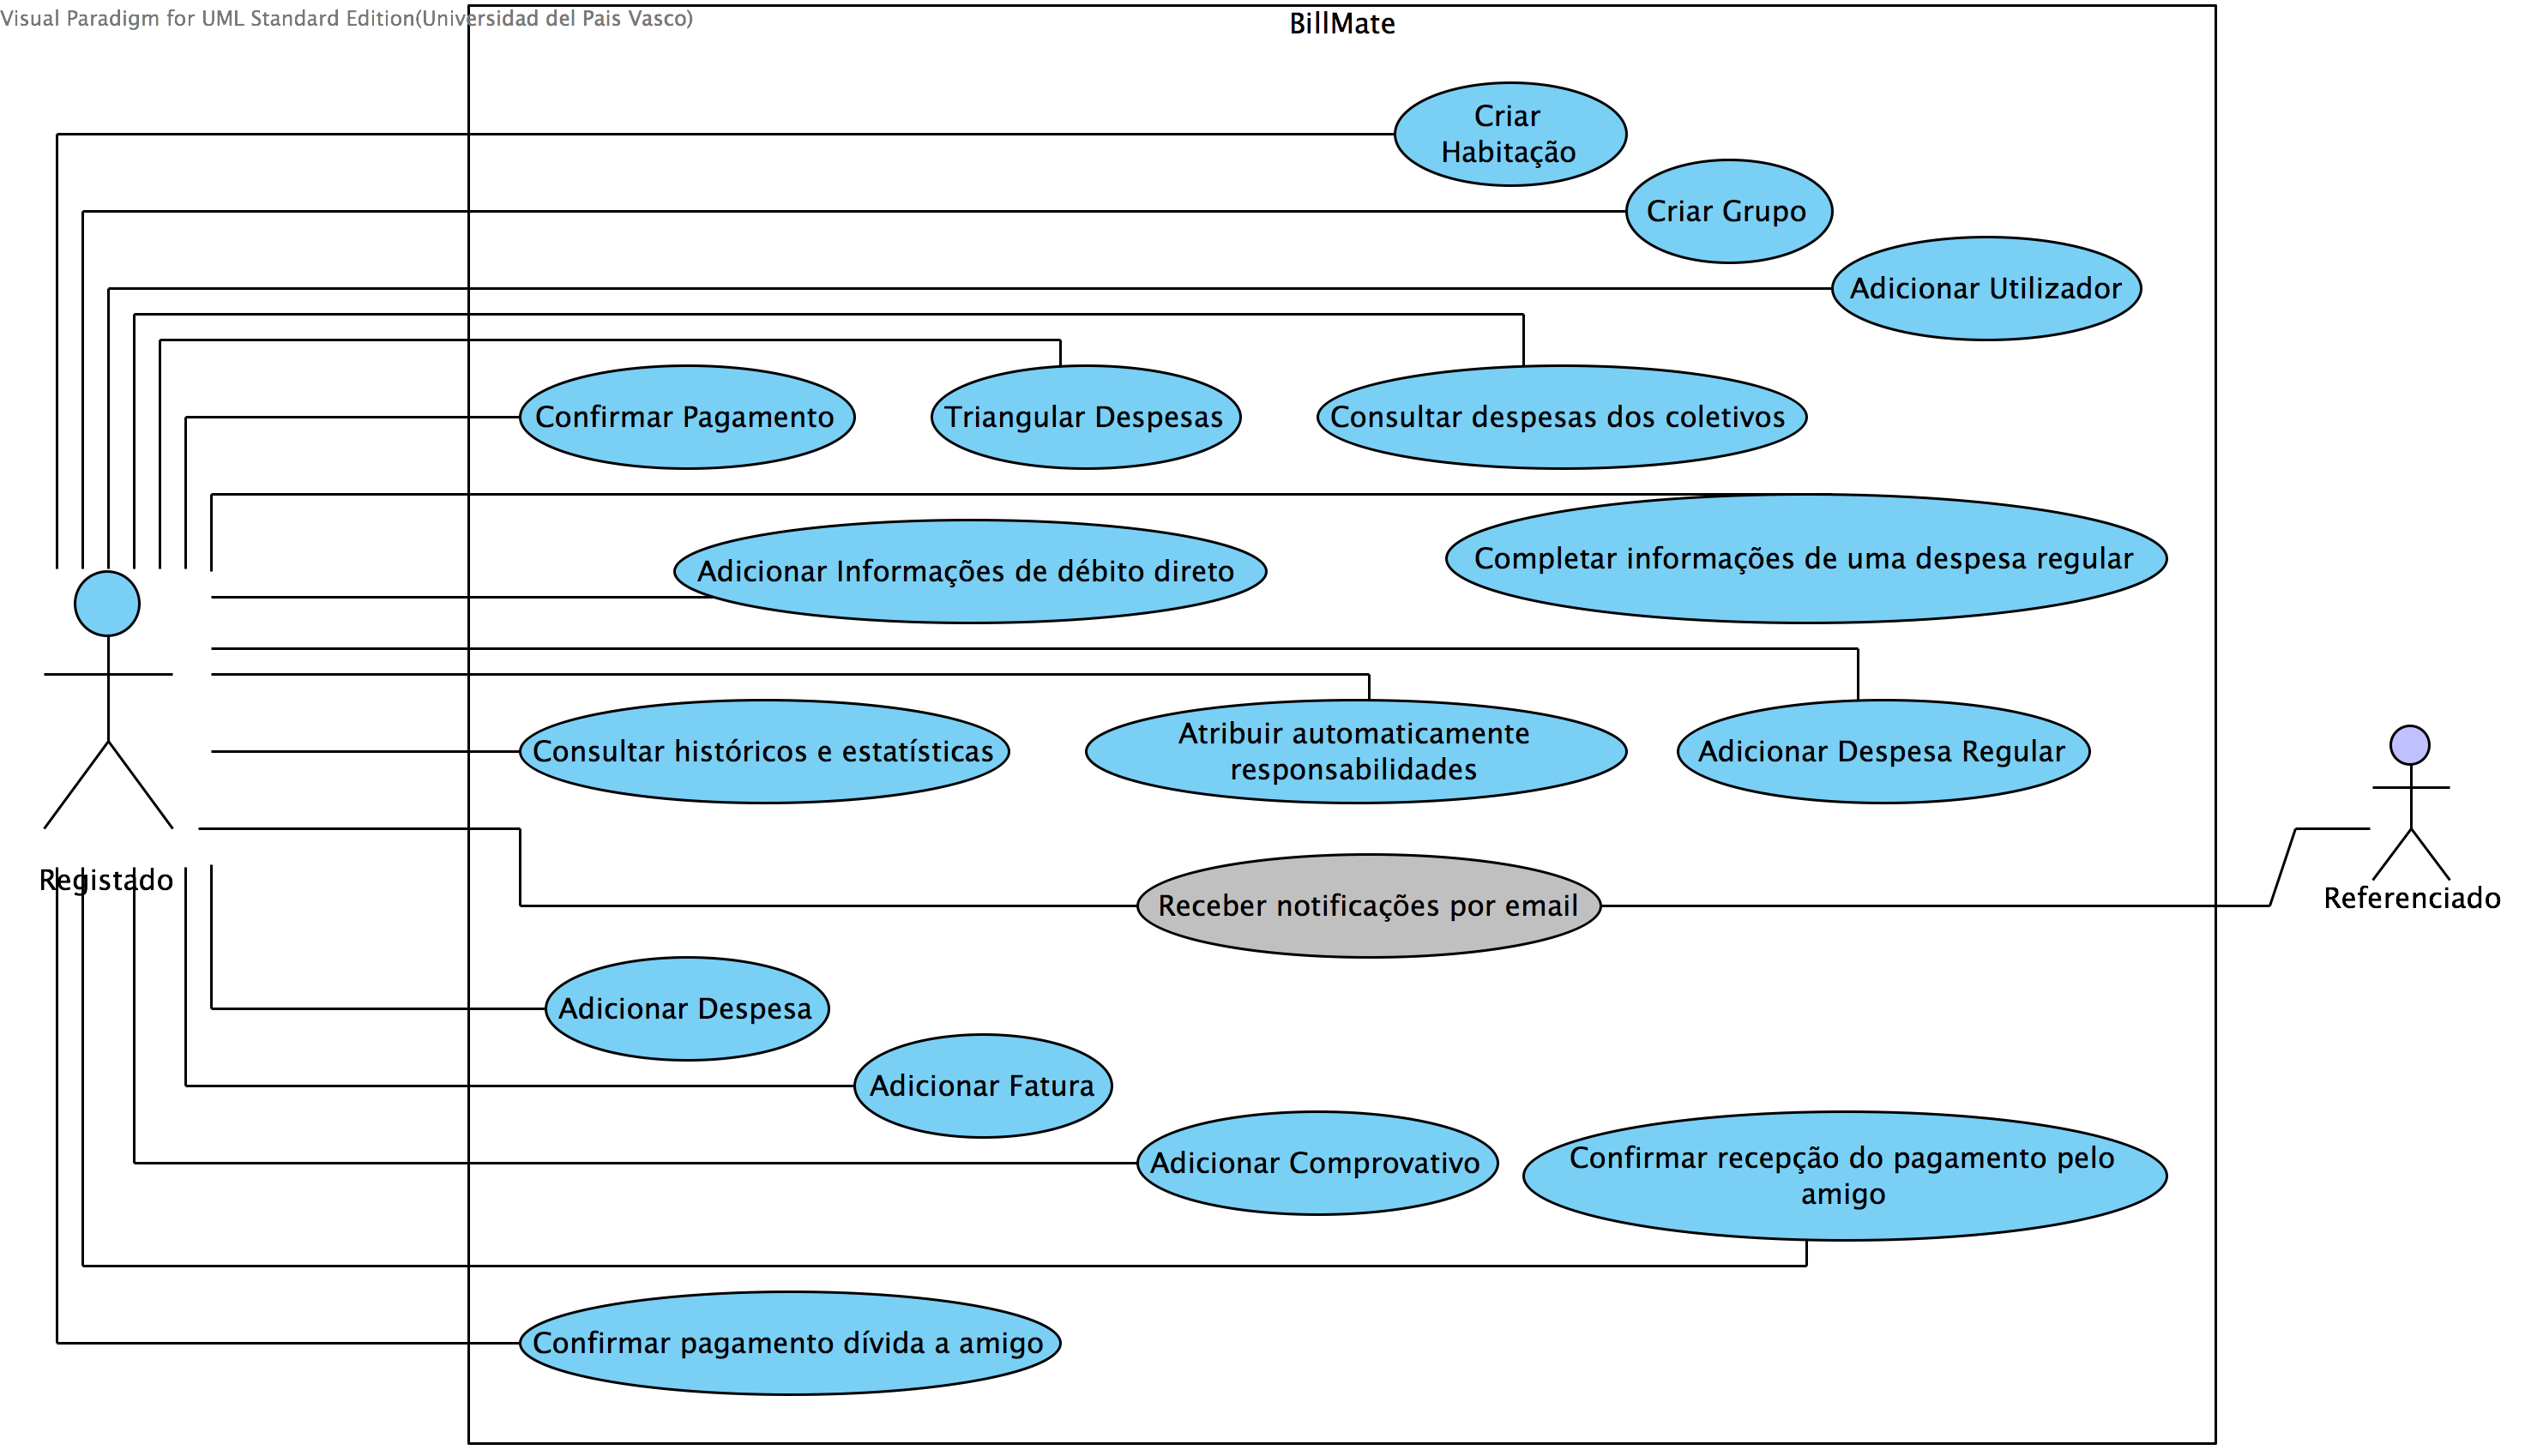
\includegraphics[width=1\textwidth]{images/modeling/useCase}}
\caption{Diagrama de use case}
\end{figure}

\section{Diagrama de Modelo de Domínio}

Tal como o próprio nome indica, domínio, é utilizado para denotar áreas funcionais dentro de sistemas que exibem funcionalidades similares. Este diagrama pode ser interpretado como sendo uma coleção de componentes de software que partilham um determinado conjunto de características.

O objetivo desta análise deve-se ao facto de se puder analisar a informação que é identificada, capturada e organizada, para que se possa reutilizar na interação entre os domínios. É certo que esta reutilização está a ser vista a um nível de abstração muito elevado, uma vez que neste momento apenas se está a analisar o domínio, mas é útil aquando da construção do diagrama de classes. Apesar de não ser este o objetivo, esta modelação será útil se for necessário que as funcionalidades sejam reutilizadas para múltiplos sistemas. \\

\begin{figure}[H]
\centerline{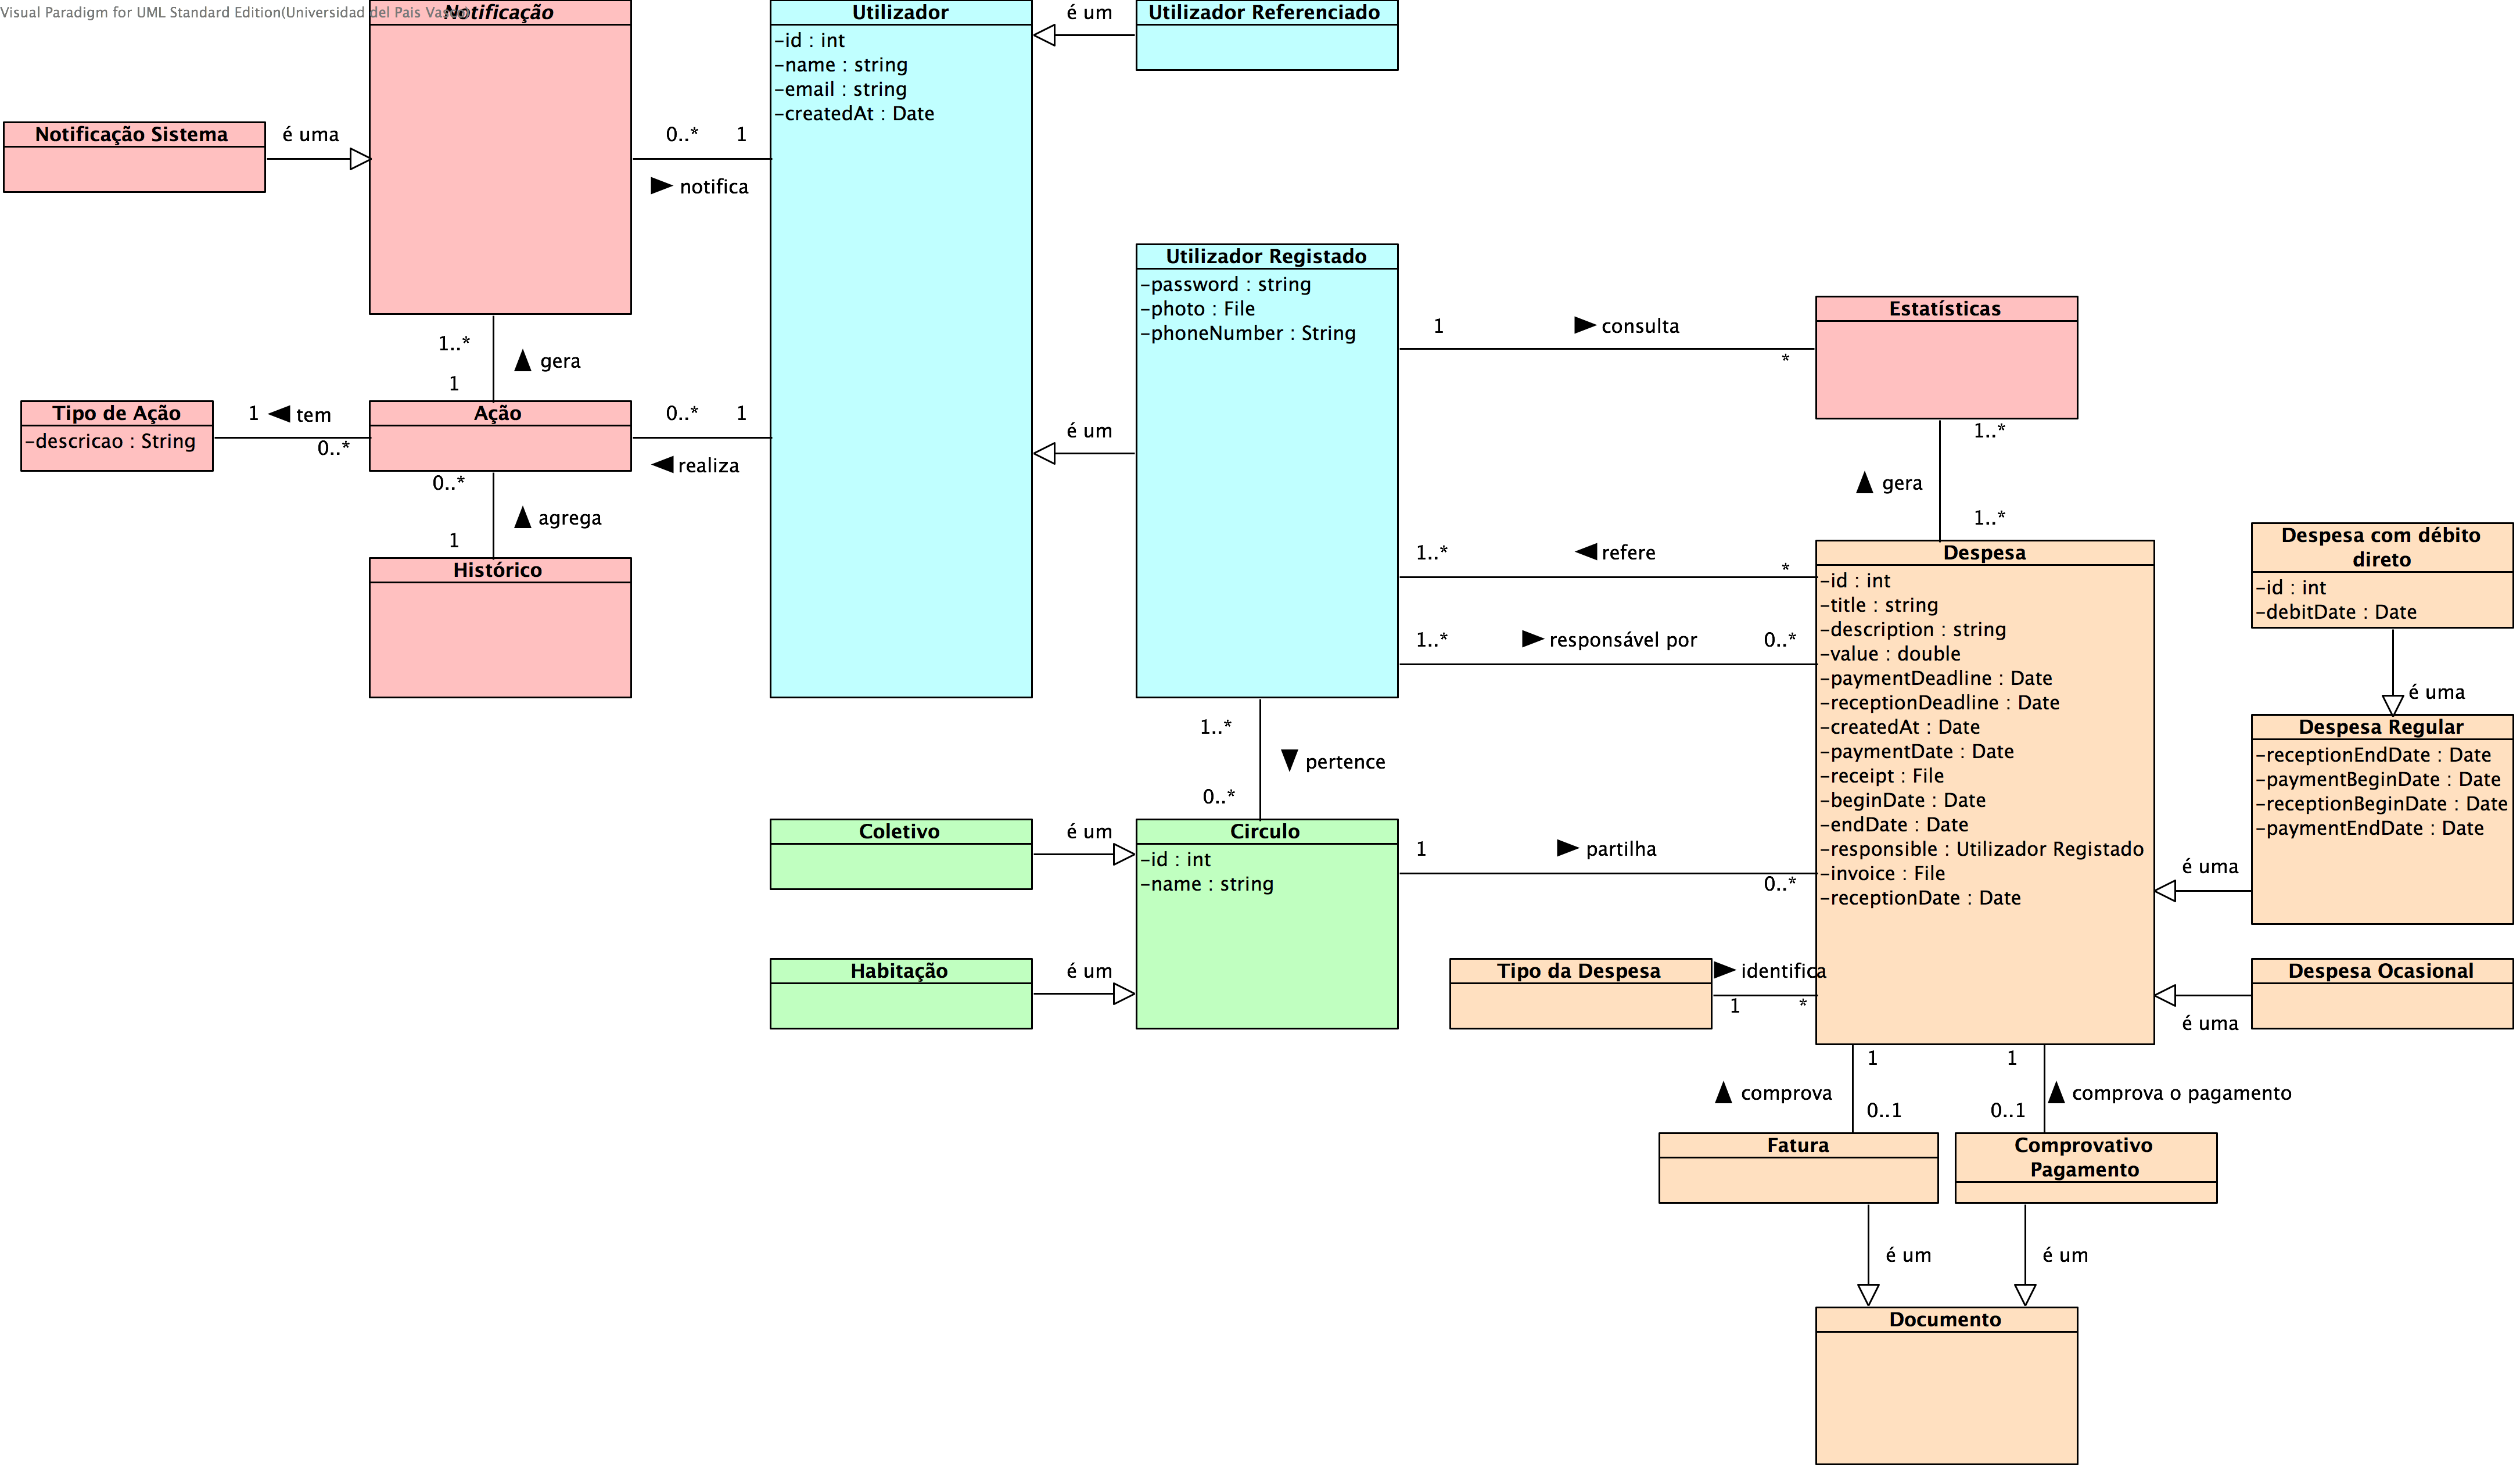
\includegraphics[width=1\textwidth]{images/modeling/modeloDominio}}
\caption{Diagrama do modelo de domínio}
\label{fig:domainModel}
\end{figure}

Tal como se pode analisar pela imagem \ref{fig:domainModel}, um utilizador é uma das entidades principais do sistema, uma vez que é este que despoleta as ações. Este utilizador pode ser classificado como registado ou referenciado. Este distinção deve-se ao facto de um utilizador não ser registado e puder ser utilizado na aplicação para partilhar despesas.
Cada utilizador encontra-se em um ou vários círculos, sendo que um círculo pode ser classificado como um tipo específico (casa), e um tipo mais genérico (colectivos).
Um determinado utilizador que se encontra em um determinado círculo tem despesas, que são partilhadas com os restantes utilizadores daquele mesmo círculo.
Definiu-se o tipo despesa no modelo de domínio, de modo a agrupar as despesas por categorias, sendo elas por exemplo, de eletricidade, de gás, entre outras, que podem até ser personalizadas.
As despesas regulares são criadas para alertar os utilizadores quando se aproxima a data de receção da fatura. Esta data, terá de ser obviamente definida pelo utilizador, que além desta data define a periodicidade com que esta se repete, normalmente mensal, mas é personalizável.
Cada despesa pode ter uma fatura e um recibo, assim como um débito direto.
Todas as ações que são feitas pelos utilizadores, geram notificações para darem feedback constante ao utilizador.

\section{Diagrama de Classes}


